%==============================================================================
%  Exam answers  --  999 Controls
%
%  To reuse for the next assignment:
%    1. copy this folder,  2. edit the METADATA block below,
%    3. edit the SOLUTIONS section,  4. run  `make`.
%
%  Build:  make          (regenerates code output, then builds main.pdf)
%          make clean    (removes build artifacts)
%==============================================================================
\documentclass[11pt,letterpaper]{article}

%------------------------------- METADATA -------------------------------------
\newcommand{\hwcourse}{EE 999 --- Introduction to Control Systems}
\newcommand{\hwcourseshort}{EE 999}  % running head, keep it short
\newcommand{\hwtitle}{Review Exam 1 --- Solutions}
\newcommand{\hwauthor}{Patrick Gordon}
\newcommand{\hwdate}{\today}
\newcommand{\hwdue}{Answers to ReviewExam1.pdf}
%------------------------------------------------------------------------------

\usepackage[T1]{fontenc}
\usepackage[utf8]{inputenc}
\usepackage{textcomp}
\usepackage[letterpaper,margin=1in,headheight=14pt]{geometry}
\usepackage{amsmath,amssymb}
\usepackage{cancel}
\usepackage{array}
\usepackage{graphicx}
\usepackage[american]{circuitikz}
\usepackage{xcolor}
\usepackage{listings}
\usepackage{fancyhdr}
\usepackage{inconsolata}
\usepackage{pdflscape}
\usepackage{float}
\usepackage[hidelinks]{hyperref}

%--- page furniture -----------------------------------------------------------
\pagestyle{fancy}
\fancyhf{}
\lhead{\hwauthor}
\chead{\hwtitle}
\rhead{\hwcourseshort}
\cfoot{\thepage}

%--- listing styles -----------------------------------------------------------
\definecolor{codebg}{HTML}{F7F7F4}
\definecolor{outbg}{HTML}{FCFCFC}
\definecolor{rule}{HTML}{C8C8C0}
\definecolor{kw}{HTML}{1C4FA1}
\definecolor{cmt}{HTML}{6A7A5A}
\definecolor{str}{HTML}{A0522D}

\lstdefinestyle{mcode}{
  language=Octave,
  basicstyle=\ttfamily\footnotesize,
  keywordstyle=\color{kw}\bfseries,
  commentstyle=\color{cmt}\itshape,
  stringstyle=\color{str},
  backgroundcolor=\color{codebg},
  frame=single,
  rulecolor=\color{rule},
  framesep=6pt,
  numbers=left,
  numberstyle=\ttfamily\scriptsize\color{gray},
  numbersep=8pt,
  showstringspaces=false,
  breaklines=true,
  columns=fullflexible,
  keepspaces=true,
  upquote=true,
}

\lstdefinestyle{moutput}{
  basicstyle=\ttfamily\footnotesize,
  backgroundcolor=\color{outbg},
  frame=single,
  rulecolor=\color{rule},
  framesep=6pt,
  showstringspaces=false,
  breaklines=true,
  columns=fullflexible,
  keepspaces=true,
  upquote=true,
}

%--- structure helpers --------------------------------------------------------
% \problem{1.1b}{Optional title}
\newcommand{\problem}[2]{%
  \bigskip
  \noindent{\large\bfseries Problem #1}%
  \ifx\relax#2\relax\else\ {\large --- #2}\fi
  \par\nobreak\vspace{2pt}\hrule\vspace{8pt}\nobreak
}

% \caplabel{Code}{hw_02_A.m}
\newcommand{\caplabel}[2]{%
  \par\nobreak\vspace{6pt}\nobreak
  \noindent{\small\bfseries #1}\ {\small\ttfamily \detokenize{#2}}%
  \par\nobreak\vspace{2pt}\nobreak
}

% \matlabcode{hw_02_A.m}  -- source listing pulled straight from the .m file
\newcommand{\matlabcode}[1]{%
  \caplabel{Code:}{#1}%
  \lstinputlisting[style=mcode]{#1}%
}

% \codeoutput{output/hw_02_A.txt} -- console output captured by the Makefile
\newcommand{\codeoutput}[1]{%
  \caplabel{Output:}{#1}%
  \IfFileExists{#1}{\lstinputlisting[style=moutput]{#1}}{\missing{#1}{run \texttt{make} to generate it}}%
}

% \answerfigure[width]{figures/foo.pdf}{Caption}  -- placeholder if not exported
% yet. Any format graphicx reads works: pdf, png, jpg.
% A script that plots is exported by the Makefile to figures/<script>.pdf, so
% \answerfigure{figures/hw_02_F.pdf}{...} is how a plotted answer is included.
% The optional argument is the printed width, default the full text width.
% Give a scan or screenshot a smaller one so it is not blown up past its own
% resolution:  \answerfigure[0.8\linewidth]{figures/some_scan.png}{...}
\newcommand{\answerfigure}[3][\linewidth]{%
  \begin{figure}[H]
    \centering
    \IfFileExists{#2}{\includegraphics[width=#1]{#2}}{\missing{#2}{export it, see README}}
    \caption{#3}
  \end{figure}%
}

% \splane{G_1(s)}  -- an empty s-plane grid to sketch poles (x) and zeros (o)
% on by hand. One unit per square, Re from -10 to 3 and Im from -4 to 4.
% \splane[5]{G_2(s)} instead centres the origin, both axes running -5 to 5.
\newcommand{\splane}[2][]{%
  \ifx\relax#1\relax
    \def\spxmin{-10}\def\spxmax{3}\def\spymax{4}\def\spxlabels{-10,-8,...,2}\def\spylabels{-4,-2,2,4}\def\spscale{1}%
  \else
    \def\spxmin{-#1}\def\spxmax{#1}\def\spymax{#1}\def\spxlabels{-#1,...,-1,1,2,...,#1}\def\spylabels{-#1,...,-1,1,2,...,#1}\def\spscale{0.85}%
  \fi
  \begin{figure}[H]
    \centering
    \begin{tikzpicture}[scale=\spscale]
      \draw[gray!30, thin] (\spxmin,-\spymax) grid (\spxmax,\spymax);
      \draw[->, thick] (\spxmin-0.3,0) -- (\spxmax+0.4,0) node[right] {$\mathrm{Re}$};
      \draw[->, thick] (0,-\spymax-0.3) -- (0,\spymax+0.4) node[above] {$\mathrm{Im}$};
      \foreach \x in \spxlabels
        \node[below, font=\scriptsize, fill=white, inner sep=1pt] at (\x,-0.05) {$\x$};
      \foreach \y in \spylabels
        \node[left, font=\scriptsize, fill=white, inner sep=1pt] at (-0.05,\y) {$\y j$};
    \end{tikzpicture}
    \caption{Pole-zero sketch of $#2$.}
  \end{figure}%
}

%--- tables -------------------------------------------------------------------
% Centred paragraph column, so a description column wraps instead of running
% off the page:  \begin{tabular}{|c|P{0.5\linewidth}|}
\newcolumntype{P}[1]{>{\centering\arraybackslash}p{#1}}

% \begin{symboltable}{Signal}{Caption}  -- the symbol / units / description
% table used to define the variables of a problem. The first argument is the
% heading of the left column (Signal, Parameter, State, ...); leave the second
% empty for no caption.
%
%   \begin{symboltable}{Signal}{}
%     \sym{x(t)}{m}{Position of tire center}
%     \sym{r(t)}{m}{Road height (depends on $v_{car}(t)$)}
%   \end{symboltable}
%
% \sym puts its first argument in math mode and brackets the units, so write
% \sym{x(t)}{m}{...}, not \sym{$x(t)$}{[m]}{...}. Anything already math -- a
% subscript, a fraction -- goes in the description as usual: $\frac{1}{4}$.
%
% The optional argument is the width of the description column, for a table
% whose descriptions are much longer or much shorter than average:
%   \begin{symboltable}[0.35\linewidth]{Parameter}{}
\newcommand{\sym}[3]{$#1$ & [#2] & #3 \\ \hline}
\newenvironment{symboltable}[3][0.45\linewidth]{%
  \def\symtabcap{#3}%
  \begin{table}[H]
  \centering
  \renewcommand{\arraystretch}{1.4}
  \begin{tabular}{|c|c|P{#1}|}
  \hline
  #2 & Units & Description \\ \hline\hline
}{%
  \end{tabular}
  \ifx\symtabcap\empty\else\caption{\symtabcap}\fi
  \end{table}%
}

% \begin{answertable}{|c|c|c|}{Caption} -- any other table. Same placement and
% captioning as \answerfigure, but you write the rows yourself:
%
%   \begin{answertable}{|c|P{0.5\linewidth}|}{Pole locations.}
%     \hline
%     Pole & Behaviour \\ \hline\hline
%     $s=-2$ & decays in half a second \\ \hline
%   \end{answertable}
\newenvironment{answertable}[2]{%
  \def\anstabcap{#2}%
  \begin{table}[H]
  \centering
  \renewcommand{\arraystretch}{1.4}
  \begin{tabular}{#1}
}{%
  \end{tabular}
  \ifx\anstabcap\empty\else\caption{\anstabcap}\fi
  \end{table}%
}

% \begin{termtable}{4}{Caption} -- collect like powers of $s$ when multiplying
% out a characteristic polynomial (or any other expansion). The argument is the
% highest power; the columns and the $s^4 \dots s^0$ header are generated from
% it, so changing the degree is a one-character edit. Leave the second argument
% empty for no caption.
%
% Cells are already in math mode: write m_1m_2, not $m_1m_2$. One row per factor
% you multiplied out, one column per power; leave a cell empty where that factor
% contributes nothing to that power. Rows end with \\, like any tabular.
%
%   \begin{termtable}{4}{Terms of the characteristic polynomial.}
%     m_1m_2 & m_1b & m_1k_s       & bk_s       & k_s(k_s+k_w) \\
%            & m_2b & m_2(k_s+k_w) & b(k_s+k_w) &              \\
%            &      & -b^2         & -bk_s      & -k_s^2
%   \end{termtable}
%
% M is a centred column that is always in math mode. It uses \( \) rather than
% $ $ so that an empty cell stays empty -- a bare $$ would start display math.
\newcolumntype{M}{>{\(}c<{\)}}
\makeatletter
\newcount\tt@i
\newcommand{\tt@cols}{}
\newcommand{\tt@head}{}
\newcommand{\tt@build}[1]{%
  \def\tt@cols{}\def\tt@head{}%
  \tt@i=#1\relax
  \@whilenum\tt@i>\m@ne\do{%
    \edef\tt@cols{\tt@cols M}%
    \ifx\tt@head\@empty
      \edef\tt@head{s^{\the\tt@i}}%
    \else
      \edef\tt@head{\tt@head & s^{\the\tt@i}}%
    \fi
    \advance\tt@i\m@ne
  }%
}
\newenvironment{termtable}[2]{%
  \def\tt@cap{#2}%
  \tt@build{#1}%
  \begin{table}[H]%
  \centering
  \setlength{\tabcolsep}{12pt}%
  \renewcommand{\arraystretch}{1.3}%
  \edef\@tempa{\noexpand\begin{tabular}{\tt@cols}}\@tempa
  \tt@head \\ \hline
}{%
  \end{tabular}
  \ifx\tt@cap\@empty\else\caption{\tt@cap}\fi
  \end{table}%
}
\makeatother

% wideproblem environment -- a problem on its own landscape page, centred.
% Use for diagrams much wider than they are tall, where a portrait page would
% shrink the labels below readable size:
%   \begin{wideproblem}{1.1b}{Title}
%     \answerfigure{figures/x.pdf}{Caption}
%   \end{wideproblem}
\newenvironment{wideproblem}[2]{%
  \begin{landscape}%
    \problem{#1}{#2}%
    \vspace*{\fill}%
}{%
    \vspace*{\fill}%
  \end{landscape}%
}

% \prompt{What special property does b*d have?} -- restate the question
\newcommand{\prompt}[1]{%
  \noindent\textit{#1}\par\vspace{6pt}%
}

% \answer{...}  -- written answer. Leave the body empty for a visible
% placeholder box; fill it in and the box is replaced by the prose.
\newcommand{\answer}[1]{%
  \ifx\relax#1\relax\todo{write the answer here}\else#1\fi
  \par\vspace{4pt}%
}

\newcommand{\todo}[1]{%
  \fbox{\parbox{0.9\linewidth}{\centering\vspace{10pt}\rmfamily\itshape\small
    #1\vspace{10pt}}}%
}

\newcommand{\missing}[2]{%
  \fbox{\parbox{0.9\linewidth}{\centering\vspace{10pt}\ttfamily\small
    missing: \detokenize{#1}\\[4pt]\rmfamily\itshape #2\vspace{10pt}}}%
}


%==============================================================================
\begin{document}

\begin{center}
  {\LARGE\bfseries \hwtitle}\\[4pt]
  {\large \hwcourse}\\[8pt]
  {\hwauthor} \quad\textbullet\quad {\hwdate}\\[4pt]
  {\small\itshape \hwdue}
\end{center}
\vspace{6pt}\hrule

%------------------------------------------------------------------------------
%  SOLUTIONS
%------------------------------------------------------------------------------

\problem{1.1(a)}{Signals and parameters}
\prompt{Model the DC motor drive of figure 1. The input is the applied voltage
$V_a(t)$; the output is the shaft position $\theta(t)$.}

\begin{symboltable}{Signal}{Signals of the DC motor drive.}
  \sym{V_a(t)}{V}{Applied armature voltage (input)}
  \sym{i_a(t)}{A}{Armature current}
  \sym{v_L(t)}{V}{Voltage across $L_a$}
  \sym{v_R(t)}{V}{Voltage across $R_a$}
  \sym{E_b(t)}{V}{Back EMF of the motor}
  \sym{T_m(t)}{N-m}{Torque produced by the motor}
  \sym{M_k(t)}{N-m}{Torque of the rotational spring}
  \sym{\theta(t)}{rad}{Shaft angle (output)}
  \sym{\dot{\theta}(t) = \omega(t)}{rad/s}{Shaft angular velocity}
\end{symboltable}

\begin{symboltable}{Parameter}{Parameters of the DC motor drive.}
  \sym{L_a}{H = V-s/A}{Armature inductance}
  \sym{R_a}{$\Omega$ = V/A}{Armature resistance}
  \sym{k_t}{N-m/A}{Motor torque constant}
  \sym{k_e}{V-s/rad}{Motor back-EMF constant}
  \sym{J}{kg-m$^2$}{Rotor and load inertia}
  \sym{k}{N-m/rad}{Rotational spring stiffness}
\end{symboltable}

\problem{1.1(b)}{Constituent equations}
\answer{
    \begin{gather}
        v_L(t) = L_a\,\frac{d i_a(t)}{dt} \\
        v_R(t) = R_a\, i_a(t) \\
        E_b(t) = k_e\,\dot{\theta}(t) \\
        T_m(t) = k_t\, i_a(t) \\
        M_k(t) = k\,\theta(t) \\
        J\ddot{\theta}(t) = M_{net}(t)
    \end{gather}
}

\problem{1.2(a)}{Free body diagram}
\answer{
    The only body is the inertia $J$. The motor torque $T_m$ acts in the
    positive $\theta$ direction, and the spring, whose far end is grounded,
    resists the rotation with torque $M_k = k\theta$.
}
\begin{figure}[H]
  \centering
  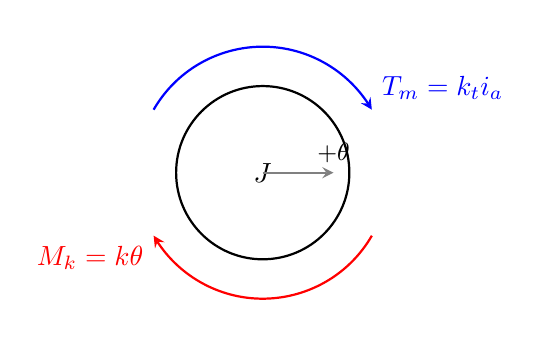
\begin{tikzpicture}[>=stealth, thick]
    \draw (0,0) circle (1.1) node {$J$};
    % motor torque, positive direction
    \draw[->, blue] (150:1.6) arc (150:30:1.6) node[above right] {$T_m = k_t i_a$};
    % spring torque, opposing
    \draw[->, red] (-30:1.6) arc (-30:-150:1.6) node[below left] {$M_k = k\theta$};
    % positive direction reference
    \draw[->, gray] (0,0) -- (0.9,0) node[above, font=\small, black] {$+\theta$};
  \end{tikzpicture}
  \caption{Free body diagram of the inertia $J$.}
\end{figure}

\problem{1.2(b)}{Continuity equations}
\answer{
    Kirchhoff's voltage law around the armature loop:
    \begin{equation}
        V_a(t) = v_L(t) + v_R(t) + E_b(t)
    \end{equation}
    Sum of torques on the inertia:
    \begin{equation}
        J\ddot{\theta}(t) = T_m(t) - M_k(t)
    \end{equation}
}

\problem{1.3}{Governing equations in standard form}
\answer{
    Substituting the constituent equations into the continuity equations:
    \begin{align}
        L_a\,\frac{d i_a(t)}{dt} + R_a\, i_a(t) &= V_a(t) - k_e\,\dot{\theta}(t) \\
        J\ddot{\theta}(t) + k\,\theta(t) &= k_t\, i_a(t)
    \end{align}
    Eliminating $i_a(t)$ (done in the frequency domain in part 4) gives a
    single third-order equation with the output on the left and the input on
    the right:
    \begin{equation}
        L_aJ\,\dddot{\theta}(t) + R_aJ\,\ddot{\theta}(t)
        + (L_ak + k_tk_e)\,\dot{\theta}(t) + R_ak\,\theta(t) = k_t\,V_a(t)
    \end{equation}
}

\problem{1.4}{Transfer function $G_{uy}(s) = \theta(s)/V_a(s)$}
\answer{
    With zero initial conditions:
    \begin{gather}
        (L_as + R_a)\,I_a(s) = V_a(s) - k_e s\,\theta(s) \\
        (Js^2 + k)\,\theta(s) = k_t\,I_a(s)
        \quad\Rightarrow\quad
        I_a(s) = \frac{Js^2 + k}{k_t}\,\theta(s)
    \end{gather}
    Substituting $I_a(s)$ into the electrical equation:
    \begin{align}
        (L_as + R_a)\,\frac{Js^2 + k}{k_t}\,\theta(s) + k_e s\,\theta(s) &= V_a(s) \\
        \Big[(L_as + R_a)(Js^2 + k) + k_tk_e s\Big]\,\theta(s) &= k_t\,V_a(s)
    \end{align}
    In rational polynomial form:
    \begin{equation}
        \boxed{G_{uy}(s) = \frac{\theta(s)}{V_a(s)}
        = \frac{k_t}{L_aJ\,s^3 + R_aJ\,s^2 + (L_ak + k_tk_e)\,s + R_ak}}
    \end{equation}
}

\problem{1.5}{Units balance}
\answer{
    Using $\mathrm{N\cdot m} = \mathrm{kg\cdot m^2/s^2}$, $[s] = 1/\mathrm{s}$
    and radians dimensionless, every term of the denominator has the same
    units:
    \begin{align*}
        L_aJ\,s^3 &: \Big[\tfrac{\mathrm{V\,s}}{\mathrm{A}}\Big]\big[\mathrm{kg\,m^2}\big]\Big[\tfrac{1}{\mathrm{s^3}}\Big]
            = \tfrac{\mathrm{V}}{\mathrm{A}}\,\mathrm{N\,m} \\
        R_aJ\,s^2 &: \Big[\tfrac{\mathrm{V}}{\mathrm{A}}\Big]\big[\mathrm{kg\,m^2}\big]\Big[\tfrac{1}{\mathrm{s^2}}\Big]
            = \tfrac{\mathrm{V}}{\mathrm{A}}\,\mathrm{N\,m} \\
        L_ak\,s &: \Big[\tfrac{\mathrm{V\,s}}{\mathrm{A}}\Big]\Big[\tfrac{\mathrm{N\,m}}{\mathrm{rad}}\Big]\Big[\tfrac{1}{\mathrm{s}}\Big]
            = \tfrac{\mathrm{V}}{\mathrm{A}}\,\mathrm{N\,m} \\
        k_tk_e\,s &: \Big[\tfrac{\mathrm{N\,m}}{\mathrm{A}}\Big]\Big[\tfrac{\mathrm{V\,s}}{\mathrm{rad}}\Big]\Big[\tfrac{1}{\mathrm{s}}\Big]
            = \tfrac{\mathrm{V}}{\mathrm{A}}\,\mathrm{N\,m} \\
        R_ak &: \Big[\tfrac{\mathrm{V}}{\mathrm{A}}\Big]\Big[\tfrac{\mathrm{N\,m}}{\mathrm{rad}}\Big]
            = \tfrac{\mathrm{V}}{\mathrm{A}}\,\mathrm{N\,m}
    \end{align*}
    The numerator $k_t$ has units $\mathrm{N\,m/A}$, so
    \begin{equation*}
        [G_{uy}] = \frac{\mathrm{N\,m}/\mathrm{A}}{\mathrm{V\,N\,m}/\mathrm{A}}
        = \frac{1}{\mathrm{V}} = \frac{\mathrm{rad}}{\mathrm{V}}
        = \frac{[\theta]}{[V_a]}
    \end{equation*}
    which are the units of output over input, so the transfer function balances.
}

\clearpage
\problem{2.1}{Governing differential equation}
\prompt{$\displaystyle G(s) = \frac{Y(s)}{U(s)} = \frac{3s + 4}{2s^2 + 14s + 20}$}
\answer{
    Cross-multiplying, $(2s^2 + 14s + 20)\,Y(s) = (3s + 4)\,U(s)$, and each
    power of $s$ is a derivative:
    \begin{equation}
        \boxed{2\ddot{y}(t) + 14\dot{y}(t) + 20\,y(t) = 3\dot{u}(t) + 4\,u(t)}
    \end{equation}
}

\problem{2.2}{Impulse response}
\answer{
    With $u(t) = \delta(t)$, $U(s) = 1$ and $Y(s) = G(s)$. In monic form with
    $K_{rlg}$:
    \begin{equation}
        Y(s) = \frac{3}{2}\,\frac{s + \frac{4}{3}}{s^2 + 7s + 10}
             = \frac{3}{2}\,\frac{s + \frac{4}{3}}{(s+2)(s+5)}
             = \frac{C_1}{s+2} + \frac{C_2}{s+5}
    \end{equation}
    By cover-up:
    \begin{align}
        C_1 &= \Big[\frac{3}{2}\,\frac{s + \frac{4}{3}}{s+5}\Big]_{s=-2}
             = \frac{3}{2}\cdot\frac{-\frac{2}{3}}{3} = -\frac{1}{3} \\
        C_2 &= \Big[\frac{3}{2}\,\frac{s + \frac{4}{3}}{s+2}\Big]_{s=-5}
             = \frac{3}{2}\cdot\frac{-\frac{11}{3}}{-3} = \frac{11}{6}
    \end{align}
    (Check: $C_1 + C_2 = \frac{3}{2}$, the leading coefficient of the monic
    numerator, as it must be for a strictly proper second-order system.)
    \begin{equation}
        \boxed{y(t) = \left(\frac{11}{6}\,e^{-5t} - \frac{1}{3}\,e^{-2t}\right)1^{+}(t)}
    \end{equation}
}

\clearpage
\problem{3.1(a)}{Reference response $T_{ry}(s)$}
\prompt{$G_c(s) = k_p$, \quad $\displaystyle G_p(s) = \frac{2s+3}{s(2s+1)}$, \quad
$\displaystyle H_y(s) = \frac{1}{0.1s+1}$}
\answer{
    Signals around the loop, with $d = 0$:
    \begin{gather}
        E(s) = R(s) - H_y(s)\,Y(s) \\
        Y(s) = G_p(s)\,G_c(s)\,E(s)
    \end{gather}
    \begin{align}
        Y(s) &= G_pG_c\big(R(s) - H_y Y(s)\big) \\
        \big(1 + G_cG_pH_y\big)\,Y(s) &= G_cG_p\,R(s) \\
        T_{ry}(s) &= \frac{G_cG_p}{1 + G_cG_pH_y}
    \end{align}
    Substituting and clearing fractions (multiply top and bottom by
    $s(2s+1)(0.1s+1)$):
    \begin{align}
        T_{ry}(s) &= \frac{k_p\,(2s+3)(0.1s+1)}{s(2s+1)(0.1s+1) + k_p(2s+3)} \\
                  &= \frac{k_p\,(0.2s^2 + 2.3s + 3)}{0.2s^3 + 2.1s^2 + (1 + 2k_p)\,s + 3k_p}
    \end{align}
    or, with monic polynomials,
    \begin{equation}
        \boxed{T_{ry}(s) = k_p\,\frac{s^2 + 11.5s + 15}{s^3 + 10.5s^2 + (5 + 10k_p)\,s + 15k_p}}
    \end{equation}
}

\problem{3.1(b)}{Disturbance to error $T_{de}(s)$}
\answer{
    With $r = 0$:
    \begin{gather}
        E(s) = -H_y(s)\,Y(s) \\
        Y(s) = G_p(s)\big(D(s) + G_c(s)\,E(s)\big)
    \end{gather}
    \begin{align}
        E(s) &= -H_yG_p\,D(s) - H_yG_pG_c\,E(s) \\
        \big(1 + G_cG_pH_y\big)\,E(s) &= -G_pH_y\,D(s) \\
        T_{de}(s) &= \frac{-G_pH_y}{1 + G_cG_pH_y}
    \end{align}
    Multiplying top and bottom by $s(2s+1)(0.1s+1)$:
    \begin{align}
        T_{de}(s) &= \frac{-(2s+3)}{0.2s^3 + 2.1s^2 + (1 + 2k_p)\,s + 3k_p}
    \end{align}
    \begin{equation}
        \boxed{T_{de}(s) = -10\,\frac{s + 1.5}{s^3 + 10.5s^2 + (5 + 10k_p)\,s + 15k_p}}
    \end{equation}
    Both transfer functions share the same closed-loop denominator,
    $1 + G_cG_pH_y$, as expected.
}

\clearpage
\problem{4}{Laplace transform vs.\ transfer function}
\begin{answertable}{|c|l|c|}{Answers to Problem 4.}
  \hline
  & Statement & Answer \\ \hline\hline
  1 & It depends on system parameters. & T.F. \\ \hline
  2 & It is determined from a time domain signal. & L.T. \\ \hline
  3 & It has an inverse. & L.T. \\ \hline
  4 & It has units. & Both \\ \hline
  5 & The time-domain function can be found by partial fraction expansion. & L.T. \\ \hline
  6 & It is a rational polynomial. & Both \\ \hline
\end{answertable}
\answer{
    \begin{enumerate}
        \item A transfer function is built from the masses, springs,
              resistances and so on of the system. A Laplace transform is
              built from a signal, which need not come from any system.
        \item A Laplace transform is computed from a time-domain signal,
              $F(s) = \int_0^\infty f(t)e^{-st}dt$. A transfer function is
              derived from the differential equations of the system.
        \item The inverse of a Laplace transform is the original time-domain
              signal. A transfer function describes a system, not a signal,
              so there is no time function it is ``the transform of'' (Part
              3b, section 10).
        \item A Laplace transform of $x(t)$ in meters has units of
              meter-seconds. A transfer function has the units of output over
              input, for example rad/V in Problem 1.
        \item Partial fraction expansion is the inverse Laplace transform:
              it breaks $Y(s)$ into table entries to recover the signal
              $y(t)$. (A transfer function is only expanded this way once it
              has been multiplied by an input to form $Y(s) = G(s)U(s)$, as
              with the impulse in Problem 2.)
        \item Both are ratios of polynomials in $s$: the transfer function
              comes from the coefficients of the differential equation, and
              every elementary signal in the Laplace table has a rational
              transform.
    \end{enumerate}
}

\clearpage
\problem{EC}{Dynamic equivalent}
\answer{
    Using the Firestone analogy (velocity $\leftrightarrow$ voltage, force
    $\leftrightarrow$ current, mass $\leftrightarrow$ capacitance,
    damper $\leftrightarrow$ conductance $1/R$, spring $\leftrightarrow$
    inverse inductance $1/L$), each mass becomes a node whose voltage is its
    velocity, with a capacitor from that node to ground (the inertial
    reference).
    \begin{enumerate}
        \item Components:
            \begin{enumerate}
                \item Resistors: \textbf{2} --- $b_1$ (to ground) and $b_2$ (between the masses).
                \item Capacitors: \textbf{2} --- $M_1$ and $M_2$.
                \item Inductors: \textbf{1} --- $k_2$.
            \end{enumerate}
        \item \textbf{Two} non-ground nodes, one per mass:
              $v_1 = \dot{x}(t)$ and $v_2 = \dot{y}(t)$.
        \item The applied force $f(t)$ becomes a \textbf{current source}
              $i_s(t) = f(t)$ driving node 1 from ground.
        \item The schematic is shown in figure~\ref{fig:ec}.
        \item Component values:
    \end{enumerate}
}
\begin{answertable}{|c|c|c|}{Component values of the equivalent circuit.}
  \hline
  Component & Value & Connected between \\ \hline\hline
  $i_s(t)$ & $f(t)$ & ground $\to$ node 1 \\ \hline
  $C_1$ & $M_1$ & node 1 -- ground \\ \hline
  $R_1$ & $1/b_1$ & node 1 -- ground \\ \hline
  $L_2$ & $1/k_2$ & node 1 -- node 2 \\ \hline
  $R_2$ & $1/b_2$ & node 1 -- node 2 \\ \hline
  $C_2$ & $M_2$ & node 2 -- ground \\ \hline
\end{answertable}
\begin{figure}[H]
  \centering
  \begin{circuitikz}
    % node 1: applied force, mass M1, friction to base
    \draw (0,0) to[I, l=${i_s = f(t)}$] (0,4)
      -- (2.7,4) to[C, l_=${C_1 = M_1}$] (2.7,0);
    \draw (2.7,4) -- (5.5,4) to[R, l_=${R_1 = 1/b_1}$] (5.5,0);
    % vibration damper: spring and damper in parallel between the masses
    \draw (5.5,4) -- (7.5,4) to[R, l^=${R_2 = 1/b_2}$] (10.8,4);
    \draw (7.5,4) -- (7.5,6.5)
      to[L, l=${L_2 = 1/k_2}$] (10.8,6.5) -- (10.8,4);
    % node 2: damper mass M2
    \draw (10.8,4) -- (11.8,4) to[C, l=${C_2 = M_2}$] (11.8,0);
    % reference node: zero velocity
    \draw (0,0) -- (11.8,0);
    \draw (5.5,0) node[ground]{};
    \draw (7.5,4) node[circ]{} node[above left]{$v_1 = \dot{x}$};
    \draw (10.8,4) node[circ]{} node[above right]{$v_2 = \dot{y}$};
  \end{circuitikz}
  \caption{Firestone-analogous circuit of the mass with passive vibration damper.}
  \label{fig:ec}
\end{figure}
\answer{
    Check by node equations. KCL at node 1 and node 2:
    \begin{align}
        f &= C_1\dot{v}_1 + \frac{v_1}{R_1} + \frac{1}{L_2}\int (v_1 - v_2)\,dt + \frac{v_1 - v_2}{R_2} \\
        0 &= C_2\dot{v}_2 + \frac{1}{L_2}\int (v_2 - v_1)\,dt + \frac{v_2 - v_1}{R_2}
    \end{align}
    which, with $v_1 = \dot{x}$, $v_2 = \dot{y}$ and the values above, are
    exactly the equations of motion of the two masses:
    \begin{align}
        M_1\ddot{x} + b_1\dot{x} + k_2(x - y) + b_2(\dot{x} - \dot{y}) &= f(t) \\
        M_2\ddot{y} + k_2(y - x) + b_2(\dot{y} - \dot{x}) &= 0
    \end{align}
}

\end{document}
